%\documentclass{acm_proc_article-sp}
\documentclass{sig-alternate}


\makeatletter
\let\@copyrightspace\relax
\makeatother

\usepackage{amssymb}
\usepackage{graphicx}
\usepackage{color}


\begin{document}

\title{Good Intentions}
\subtitle{Intent-based Vulnerabilities on the Android Platform}

\numberofauthors{1} %  in this sample file, there are a *total*
% of EIGHT authors. SIX appear on the 'first-page' (for formatting
% reasons) and the remaining two appear in the \additionalauthors section.
%
%
%
\author{
% You can go ahead and credit any number of authors here,
% e.g. one 'row of three' or two rows (consisting of one row of three
% and a second row of one, two or three).
%
% The command \alignauthor (no curly braces needed) should
% precede each author name, affiliation/snail-mail address and
% e-mail address. Additionally, tag each line of
% affiliation/address with \affaddr, and tag the
% e-mail address with \email.
%
% 1st. author
\alignauthor
\small
Jonathan Graff
\& Eugene Ma
\& Ahir Reddy
\& Dominique Canlas
\& Justin Ng
\& Calvin Hu
%\alignauthor
%Bob
       }

%\author{
%% You can go ahead and credit any number of authors here,
%% e.g. one 'row of three' or two rows (consisting of one row of three
%% and a second row of one, two or three).
%%
%% The command \alignauthor (no curly braces needed) should
%% precede each author name, affiliation/snail-mail address and
%% e-mail address. Additionally, tag each line of
%% affiliation/address with \affaddr, and tag the
%% e-mail address with \email.
%%
%% 1st. author
%\alignauthor
%Ben Trovato\titlenote{Dr.~Trovato insisted his name be first.}\\
%       \affaddr{Institute for Clarity in Documentation}\\
%       \affaddr{1932 Wallamaloo Lane}\\
%       \affaddr{Wallamaloo, New Zealand}\\
%       \email{trovato@corporation.com}
%% 2nd. author
%\alignauthor
%G.K.M. Tobin\titlenote{The secretary disavows
%any knowledge of this author's actions.}\\
%       \affaddr{Institute for Clarity in Documentation}\\
%       \affaddr{P.O. Box 1212}\\
%       \affaddr{Dublin, Ohio 43017-6221}\\
%       \email{webmaster@marysville-ohio.com}
%% 3rd. author
%\alignauthor Lars Th{\o}rv{\"a}ld\titlenote{This author is the
%one who did all the really hard work.}\\
%       \affaddr{The Th{\o}rv{\"a}ld Group}\\
%       \affaddr{1 Th{\o}rv{\"a}ld Circle}\\
%       \affaddr{Hekla, Iceland}\\
%       \email{larst@affiliation.org}
%\and  % use '\and' if you need 'another row' of author names
%% 4th. author
%\alignauthor Lawrence P. Leipuner\\
%       \affaddr{Brookhaven Laboratories}\\
%       \affaddr{Brookhaven National Lab}\\
%       \affaddr{P.O. Box 5000}\\
%       \email{lleipuner@researchlabs.org}
%% 5th. author
%\alignauthor Sean Fogarty\\
%       \affaddr{NASA Ames Research Center}\\
%       \affaddr{Moffett Field}\\
%       \affaddr{California 94035}\\
%       \email{fogartys@amesres.org}
%% 6th. author
%\alignauthor Charles Palmer\\
%       \affaddr{Palmer Research Laboratories}\\
%       \affaddr{8600 Datapoint Drive}\\
%       \affaddr{San Antonio, Texas 78229}\\
%       \email{cpalmer@prl.com}
%}
% There's nothing stopping you putting the seventh, eighth, etc.
% author on the opening page (as the 'third row') but we ask,
% for aesthetic reasons that you place these 'additional authors'
% in the \additional authors block, viz.
%\additionalauthors{Additional authors: John Smith (The Th{\o}rv{\"a}ld Group,
%email: {\texttt{jsmith@affiliation.org}}) and Julius P.~Kumquat
%(The Kumquat Consortium, email: {\texttt{jpkumquat@consortium.net}}).}
\date{May 9, 2012}
% Just remember to make sure that the TOTAL number of authors
% is the number that will appear on the first page PLUS the
% number that will appear in the \additionalauthors section.

\maketitle
\begin{abstract}
    In this paper we investigate Intent-based attack surfaces on the Android
    platform. We address exploits in two ways, focusing on both detection and prevention. First, we implemented a
    static analysis tool which reports vulnerabilities in an input file. Secondly, we implemented an Android
    library which provides a mechanism for restricting the origin of intents to trusted applications.
\end{abstract}

\section{Background}

\paragraph{Activity Hijacking}
Activity Hijacking happens when an Intent is sent out implicitly and a malicious attacker happens to filter that Intent. For example, in an application where a user searches for a product on Amazon, and the application opens up the Amazon search results in a browser, the hijacker will intercept the URL before passing the intent to the real browser. The attacker can now track user activity and any data associated with the URL. Another form of attack is when an application imitates the UI and name of a trusted application. The user is presented by the OS a choice of which application to use. Once the user accidentally chooses the malicious app, the attacker is now in control of all the data being sent through Intents.

\paragraph{Service Hijacking}
Service hijacking attacks have the potential to be especially problematic because services are run in the background, so the user will have no idea that anything is wrong. They are much more difficult to pull off than other types of hijacking attacks, but the result can be worse. This is because when multiple services can handle an intent the system resolves the destination not by prompting the user, but rather based on which app was installed first. However, it is still possible for an attacker to get a malicious app onto the phone before the legitimate app, in which case it would intercept any and all relevant intents and could access data, spoof results, or cause all kinds of crazy shenanigans.

\paragraph{Broadcast Hijacking}
Broadcasted Intents can easily be captured by malicious application/component
when the right precautions are not made. Specifically, Android Broadcasts that
does not require Receiver signature or those that fail to set the Receiver
priority in the manifest can easily be manipulated by malicious software.
Broadcast Hijacking attacks can range from a simple Denial of Service to a more
serious case of Data Theft.

\paragraph{Activity Intent Spoofing}
When an application leaves its activities public or exported, it is then open to accept Intents from outside the application. This leads to attackers being able to send malformed data or request to an Activity. Depending on the tasks that an Activity performs, the attacker can make an app behave erroneously. The problem here is that the receiver of the Intent has no way of verifying if the Intent came from a trusted source.

\paragraph{Android Service Intent Spoofing}
Like spoofing activities, a service that is exported or left public can be manipulated or called by an outside application. Malicious components can bind to a service by sending an implicit Intent and exploit all its capabilities. Additionally, malicious information can be fed into the service that may cause it to die or behave unexpectedly.

\paragraph{Broadcast Intent Spoofing}
A spoofed broadcast Intent involves crafting an Intent that is broadcasted to a
victim application's BroadcastReceiver component in an attempt to feed it
malicious information or otherwise trigger unintended behavior.
BroadcastReceivers, by their nature, need to be made publicly accessible, so
they are often an obvious choice for an attack method. If a BroadcastReceiver
needs to receive Intents outside of its own package, it must declare
exported="true", making it a candidate for a spoofing attack victim. The
effectiveness of this attack depends entirely upon what sort of functionality
is contained within the victim BroadcastReceiver.  The only broadcast Intents
that cannot be spoofed are system Intents with actions such as
"ACTION\_BATTERY\_LOW," which only the Android OS can send. However,
BroadcastReceivers can always be triggered to by the use of an explicit Intent,
which explicitly specifies what component it wants to target.

\paragraph{The Goals}
The Initial goal was for the group to create a solution to the above problems. The first solution, focusing on prevention, is to create a secure library that will abstract away Intents to developers. After further analysis however of the Android architecture, it was proven that the API provides secure ways to handle most of the problems above. Those ways are described below. What is lacking, however, is a way to verify Intent origin to prevent against spoofing attacks. We therefore focused on developing a library that developers can use in order to verify Intent origin. Secondly, focusing on detection, is an analysis tool that uses inter-procedural control flow that tracks any delivered Intent. The tool also warns the user regarding the safety of an Intent (e.g. explicit or implicit). 

\section{Good Intentions Library}

\paragraph{Activity Hijacking}
Preventing Activity Hijacks are simple. A developer just needs to make sure that
the startActivity call contains an explicit Intent especially if the intent
contains private information. This will guarantee that the intent will only be
read or received by the intended receiver. If sending an implicit intent, the
contents of the intent should not contain confidential data. 

\paragraph{Service Hijacking}
Like other security problems, there are multiple ways to prevent malicious
applications from using your service. First, in the <service> tag in the
manifest, you can specify properties such as the permission required to start/bind to
the service. Next, by not defining intent filters your service can only be
started by an explicit intent. This prevents outside applications that you do
not trust from accessing it. Additionally, to ensure that your service is
private to your application, you should set the "exported" attribute in the
manifest to false.

\paragraph{Broadcast Hijacking}
Android specifies the security implications of sending Broadcasts and it
provides a robust API to mitigate or eliminate security problems in its
documentation. The following mechanisms can and should be used to prevent
Intent exploits:

\begin{itemize}
    \item{LocalBroadcastManager} - This class is to be used when you are
        sending broadcasts inside your application. It guarantees that the
        broadcasted intent does not leave your application.

    \item{sendBroadcast(Intent, receiverPermission) and the like} - When
        sending broadcasts, this enforces receiverPermission be declared
        through the <uses-permission> tag in the manifest by the
        broadcastReceiver that wants to receive an intent. when sending
        broadcasts. 

    \item{registerReceiver} - Supplying a non-null permission when registering
        a receiver restricts the broadcasted Intents that will be received to
        those matching the permission. 

    \item{Intent Spoofing (Activities, Services, Broadcasts)} - All these three
        have similar solutions. If a developer does not intend the component to
        receive external Intents, the above components can be made private to
        the app by declaring the "exported" attribute to be false. Otherwise,
        the developer needs to check the caller's identity of the Intent or
        verify that the Intent received is not malicious.  Android, however,
        does not provide a way to verify the origin of an Intent. But, if a
        developer knows which applications or components to trust, we can then
        verify the origin of the intent before receiving it.  This solution is
        described in depth below.
\end{itemize}
Based on all these analyses we see that Android provides a secure API for
application developers to prevent malicious attackers. It is almost always the
developer's responsibility to make sure that the application is secure and that
methods being used to send Intents are the appropriate ones for the type of
data being sent. Furthermore, because the intent system is so flexible it is very difficult to 
distinguish between legitimate and malicious functionality. 
Any attempt to create a comprehensive “secure library” would thus consist of little more than renaming methods that already exist! 

\Section{Final Method/Solution & Justification for design}
We therefore decided to fully shift our focus to a functionality that we had
originally conceived of as part of the library. The idea is to provide a
mechanism for components that receive intents to restrict what apps they will
accept intents from. One cause of potential security vulnerabilities that we
identified was the fact that Android does not provide origin information for
Intents. This can be problematic in cases where a component is intended to
provide sensitive functionality for a known subset of external applications,
but must not be used by untrusted apps. In the absence of origin information
Intents can be easily spoofed, causing the target app to leak data, give
malicious apps unauthorized permissions, or be subject to any other
Intent-based exploit. We set out to prevent this.

Because modifying the Android OS was beyond the scope of this project, we had
to think creatively about possible solutions within the existing framework. We
carefully considered a lot of different ways to do this, and finally settled on
the following model because it provides the best balance of ease of use and
security. The idea is that a receiving component can define a list of trusted
packages, and will only respond to intents from components within them by
requiring some form of identification. Note that any mechanism that relies on
secret keys will not work, as an attacker can simply decompile the code to
obtain it. The key must be generated randomly and sent to authorized apps. We
do this by taking advantage of one of the most fundamental Android security
guarantees - that an explicit intent will reach its target without being
intercepted - to allow the receiving component to give keys to only those apps
it trusts.  

Our system was designed to be easily usable, without requiring the developer to
understand anything about how it works. All they need to do is extend an
abstract class and register a component in the manifest. The functionality is
implemented in the form of two abstract Service classes, to be extended by the
developer in both the sending and receiving apps. These are called the
Solicitor (sender) and the Bouncer (receiver). The components that use these to
communicate will be referred to as the sending and receiving components. The
developer of the receiving component must extend the Bouncer, register it as a
service, and implement an abstract method specifying which packages should be
trusted. The receiving component must not be exported; it will only receive
intents through the Bouncer. The developer of the sending component must do the
same for the Solicitor, extending and registering it. When the sending
component wishes send an Intent to the receiving component, it simply calls a
method in its local Solicitor and everything is taken care of securely. 
When the Solicitor is invoked it is passed the Intent object that the sending
component wishes to send to the receiver. It stores the object in memory for
later use and then begins the process by contacting the receiving app's Bouncer
with a normal call to startService(). Contained in this call is origin
information provided by the Solicitor, which is then checked by the Bouncer
against its list of authorized packages. If the check passes, the Bouncer then
binds to the Solicitor Service explicitly. The Solicitor uses the binding
interface to send along the original intent, which the Bouncer passes along to
the receiving component.

We will now discuss what makes this system secure. Most importantly, the
receiving component is not exported, which means that only components within
the same package can contact it. This ensures that all communication must go
through the developer's extension of our Bouncer class, which is in the same
package. The Bouncer will only forward Intents to the receiver after it has
determined that it is from a trusted package, which is achieved through the
combination of checking the origin info against a list and binding to it
explicitly. It is important to note that the check itself provides no security,
as the origin field can be easily spoofed. The security guarantee comes from
the fact that the Bouncer binds to the Solicitor explicitly, which means it
specifically targets the trusted package. The Android system can be trusted to
carry this out without the possibility of interception. If a malicious app
spoofs the origin package, the Bouncer will end up binding to a trusted app's
Solicitor, which will simply refuse the connection because it knows it has no
pending requests. Security is thus ensured. We successfully devised and
implemented a system that provides a guarantee of origin for Intents.

\section{Usage}
To use this intent proxy system, the developers of the two applications must
agree to allow communication between their components.  Both parties import the
intent proxy library in their projects.  If application A wants to send intents
targeted at application B's components, A will fill out a stub class
"DevAppSolicitorImpl" which extends the Solicitor class.

And application B will fill out a stub class "DevAppBouncerImpl" which extends
the Bouncer class.  Here, B must implement the setTrustedPackages() method, and
add trusted package names to the trustedPackages field.

When A wants to send B an intent, it will craft an intent as usual, but instead
of launching it with the Android's conventional methods (e.g.
startActivity()), it will call one of our safe static methods,
safeStartActivity(), safeStartService(), or safeSendBroadcast(), defined in the
GIProxy class.

\section{Static Analysis}
\subsection{Introduction}
Our goal is to write a static analysis tool that warns the user about any
potentially dangerous Intents that could be sent by the target application.
IntentAnalyzer is a command line tool written in Python that performs such
analysis. IntentAnalyzer uses inter-procedural control flow analysis to track
all delivered Intents. Information about delivered Intents helps IntentAnalyzer
decide if the application is sending Intents safely. For instance,
IntentAnalyzer is able differentiate between implicit and explicit Intents by
checking whether or not the Intent contains a Component field. By default,
IntentAnalyzer flags all implicit Intents as dangerous.

\subsection{Approach}
To begin, we had to decide on a data structure which would suit our purposes
for analyzing the control flow of a program. We researched existing static
analysis frameworks, and decided to use a \emph{control flow graph} to
represent execution flow. We followed a set of distinct steps is to construct a
control flow graph from a raw dex file.

%The first step is to parse the dex file into
%internal data structures representing individual methods and instructions. The
%second step is separating the instruction stream into basic blocks. The third
%step is to build a intra-procedural control flow graph, using basic blocks as
%vertices in this graph. Finally, we need to combine these intraprocedural
%graphs into a single graph encapsulating control flow across method calls.

\paragraph{Parsing}
While Java programs are compiled and run in a Java VM, Android programs are run
using a Dalvik VM. This means that a Dalvik Executable is generated by the
Android compiler (.dex extension) which allows the Dalvik virtual machine to
run the application. This .dex file is packaged in Android .apk file. To make
our task easier, we used a customized version of DexDump to process a raw dex
file into an XML format.  Our project utilizes this existing dex to XML
converter, which separates classes, methods, and instructions into XML tags.
Since Python already includes a rich library for parsing XML, converting the
XML into native Python data structures and custom classes was an easy task.

%From this point, the xml file is parsed into a graph structure, consisting of
%basic blocks grouped by method signature. The first step is separating each
%instruction into basic blocks.  Since most instructions tend to execute
%sequentially, it is more efficient to group instructions together into bundles
%called basic blocks. 

\paragraph{Basic Blocks}
The next task is to separate instructions into basic blocks. Basic blocks
constitute the "nodes" of our analyzer - each basic block is a consecutive set
of instructions that consists of one entry point and one exit point. When the
first instruction of a basic block is executed, the rest of the instructions in
the block are always executed in order. We wrote a subroutine which takes in an
instruction stream, and outputs an ordered list of basic blocks. Basic blocks
are created by examining the instruction stream, and marking instructions which
start new basic blocks, such as jump targets, or instructions that follow
untaken branches. Then the instructions are separated into basic blocks by
emitting a new basic block every time a new entry point instruction is
encountered.

\paragraph{Intraprocedural Graph}
Now that we have basic blocks, each basic block is connected to the appropriate
successor basic blocks. The connectivity for each basic block depends on the
last instruction. For instance, basic blocks that end with a branching
instruction may have multiple successors blocks. We implemented this approach
by creating a mapping between basic blocks and jump targets. Basic block nodes
which end with method invocations are simply connected to the next sequential
basic block at this step, but are expanded in the next step.

%In this way, paths through the graph
%represent distinct instruction execution paths; thus, by constructing the graph
%with basic blocks we can enumerate all possible flows of execution through the
%program. 

\paragraph{Interprocedural Graph}
Initially, we construct a control flow graph for each method. Starting with an
entry point method, we "expand" method invocation nodes until the graph reachs
a fixed point. From here, we identify the entry point methods (for example
Android activities start with onCreate). For each entry point method, each
method call in the graph is unrolled, in essence creating a union of the graph
of the caller and callee method. For every basic block node which ends with an
invoke instruction, we delete the edge between that node and the next node.
Then we create a copy of the callee's control flow graph. The node that invokes
a method is connected to the entry point of this new graph (the first
instruction). The basic block that makes a call to a method is now linked to a
new instance of the entry basic block of the method. All return statements in
the called method are then linked back to the basic block that immediately
follows the calling basic block (a directed edge points out of the return
statement blocks). In essence each invoke node can be "expanded" an arbitrary
amount of times. Therefore, our interprocedural analysis algorithm has an
unlimited call depth.  In particular, it is important to note that when the
same method is called multiple times, each "expansion" generates a new graph,
despite the fact that they were generated from the same method.

\paragraph{All Simple Paths}
Given a completely "expanded" graph data structure, we now can build a static
analysis algorithms on top of this framework. In particular, we want to track
intents as they are instantiated, until they are passed into a "sink", a
method which initiates the IPC process between Android components. An example
sink that launches a new Android application is startActivity, or bindService.
These sink methods take in an Intent as a parameter.

We enumerated all paths from entry points of the application, to all sinks of
the application. Each path defines a single Intent that could possibly be sent
from this application, and is essentially a sequential, ordered list of nodes,
and each node decomposes into a linear sequence of instructions. However
enumerating all non-cyclic paths in this manner can take a very long time to
complete. The running time is non-polynomial, O(n!). Therefore, some graphs can
take minutes, while others can take seconds to complete analysis.

At the end of this process, the paths represent all possible flows of execution
through the program which end with a sink. All branches are followed, giving so
an upper bound on the number of paths through the program because even
impossible branches are followed, since the tool does not perform constraint
satisfaction.

\paragraph{Transfer Functions}
The static analysis problem we wish to solve is to determine the state of the
Dalvik VM registers right before the sink is executed. Given a linear sequence
of instructions represented as a \emph{path}, we can simply follow it and
update the register state after each analyzed instruction. To accomplish this,
we wrote transfer functions for each instruction. Each instruction that was on
the path is passed a "state" data structure, which contained all register
mappings and tracked Intents. After passing through every instruction in a
path, the state would contain the register mapping right before the execution
of the sink instruction. With this information, we can check that the argument
register of the sink method contains a reference to an Intent, and output
accordingly.  For each Intent found, it contains all attributes collected along
the way, including action string, categories, extra data, target component, and
miscellaneous flags.

One challenge we had was tracking state between method calls. Even though we
expanded method calls in place, such that the new nodes and edges were
connected with the existing graph, each method call produces a  \emph{frame}
with its own registers mappings. Therefore, we represented the state of the
execution as a stack of register mappings. Mappings were pushed and popped from
the stack as invoke nodes and return nodes were encountered.

\paragraph{Intent Analysis}
At this stage, we have a list of all the Intents that were detected by our
tool. By default, our tool simply flags all implicit Intents as dangerous.
Implicit Intents do not specify a target component by the time it reaches the
sink. We classify implicit Intents as dangerous, because it renders the
application vulnerable to Activity Hijacking, Service Hijacking, and Broadcast
Theft. Any malicious app is able to intercept the Intent and read its contents
by specifying a matching Intent Filter. Admittedly, this heuristic for flagging
dangerous Intents is simple and crude, but more elaborate schemes for
identifying dangerous Intents could implemented in the future.

\subsection{Limitations}
Future revisions of the project may perform constraint analysis on branches to
reduce the number of paths, but we believed it to be outside of the scope of
the project to track conditions on branches. Similarly, a future revision will
implement tracking of switch statements. The final limitation is the
computation of all distinct paths between source and sink nodes when
enumerating all paths that create and emit intents. Currently, our search can
take O(n!) time in the worst case. This search can possibly be improved by
exploiting the properties of Directed Acyclic Graphs.

Our analysis framework is general enough to work for any method defined in the
class file, using the push and pop mechanism of register mappings to track
state across method calls. However, external methods such as library methods
need to be implemented as "stubs", because we could not actually generate their
graphs, since their implementations are not in the dex file. Stubs are Python
functions which take state and arguments as parameters, and modify them in a
predetermined way. We had to define a new stub for each library method. This is
tiresome in general, so we did not cover every single Android API call; we
covered the ones relevant to our interests, such as any Intent method which
modified the Intent in some way. Therefore, the information we collect on
Intents may be incomplete, because not all API methods are defined.

Finally, we adopted a simple heurustic for flagging dangerous intents. Intents
without components are flagged as dangerous. This could be improved in the
future by using a more precise heuristic, such as checking whether or not the
action string of the Intent is supported by the Android API, or just
internally.

\subsection{Improvements Over Comdroid}
By building the graph through iterative method unrolling overcome, our project
overcomes Comdroid's 1 level function call limit. Furthermore, our analysis
splits branches into 2 or more distinct paths that are tracked separately,
there by enumerating over paths that Comdroid does not and allowing the
discovery of vulnerable intents that Comdroid can not find. For example, if one
branch creates an implicit Intent, and another creates an explicit Intent,
ComDroid will report an explicit Intent, whereas IntentAnalyzer will report
both.


\subsection{Example Analysis}
As an example we will analyze a release of the Opera mobile web browser.
Although our tool examines all entry points, here we look at a single entry
point, \emph{onPause()}. Figure \ref{example_analysis} shows the graph that is generated
after the entry point method is expanded. By manual inspection, we can see that
block 8292 is a source node, and block 8294 is a sink node, since one allocates
a new Intent, and the other delivers it. There is only a single path from
source to destination. An Intent is created from this path and we can determine
changes to its attributes as it travels along the path. The figure demonstrates
that the tracked Intent contains an \emph{action} string and \emph{extra} data.
It is implicit because the \emph{classname} and \emph{class} fields are empty.
Thus, it is dangerous. It also appears that the action is meant for an internal
component, since the string seems to specify an Intent action string specific
to Opera. Therefore, we discovered a vulnerability in Opera after running the
dex file through IntentAnalyzer, because any malicious application could
potentially intercept this Intent and perform Broadcast Theft.

\clearpage
\begin{figure}[t!]
    \centering
    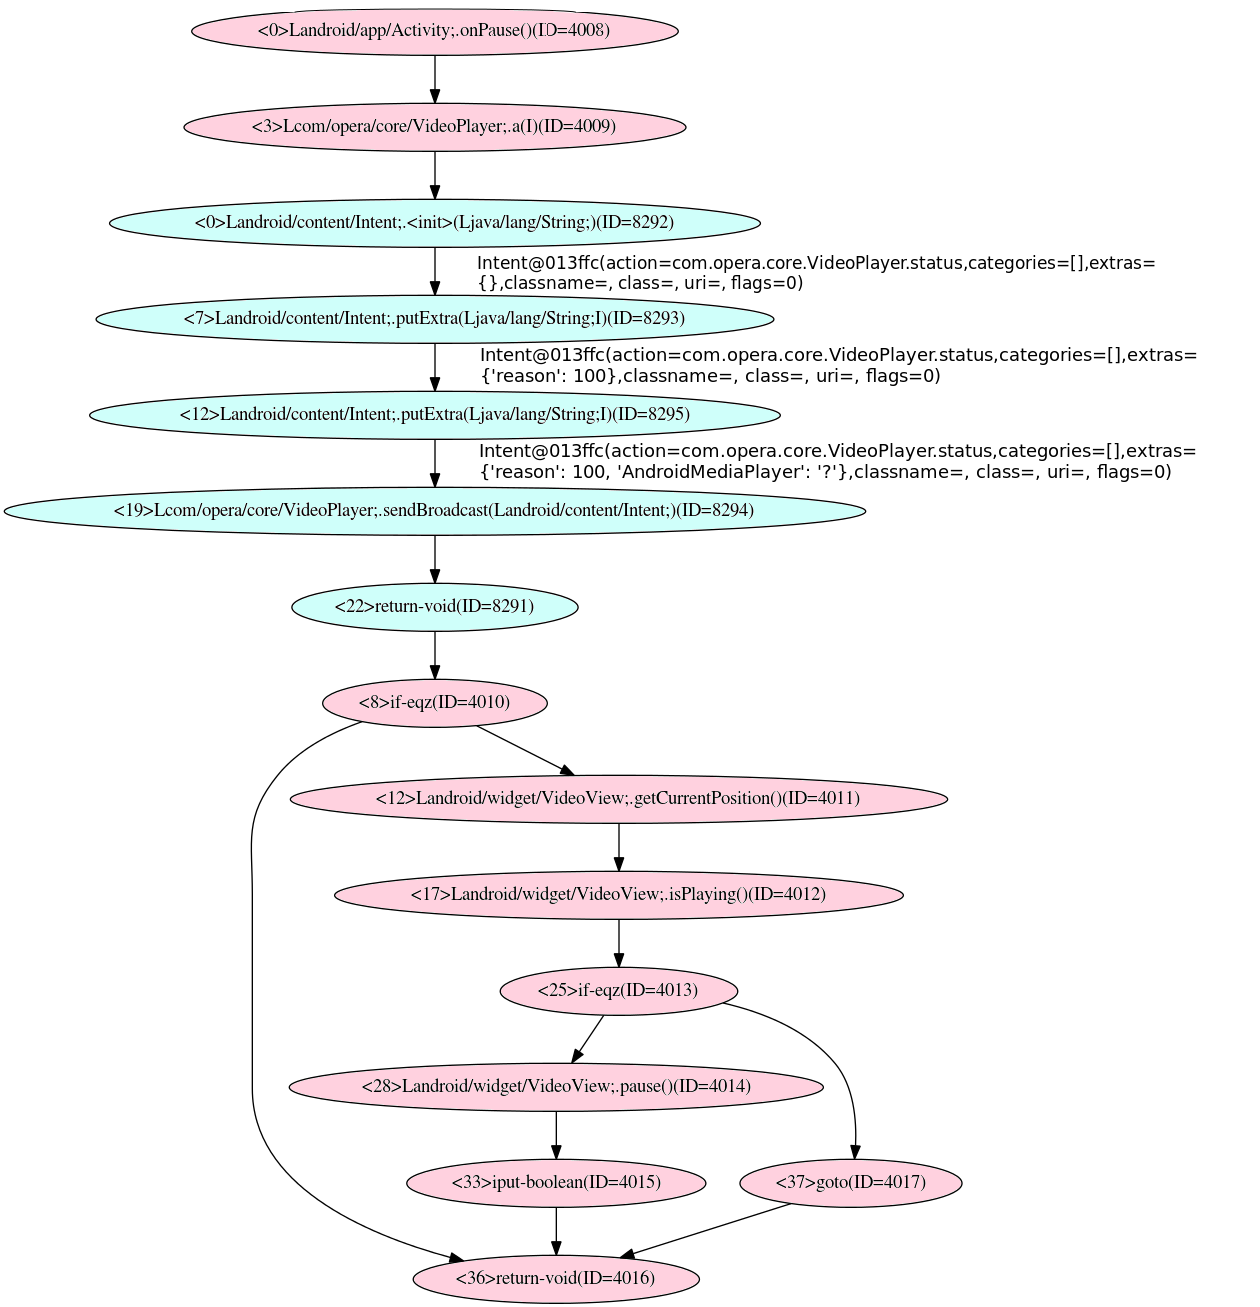
\includegraphics[width=2\columnwidth]{figures/annotated}
    \caption{This diagram shows an example control flow graph. Each node
        represents a basic block, and is labeled by the last instruction within
        that basic block. Different colored nodes represent basic blocks from
        separate methods. For example, before expansion, basic block 4009 is
        connected to basic block 4010. After expansion, we splice in the nodes
    and edges from the invoked method's graph.}
    \label{example_analysis}
    \vspace*{6in}
\end{figure}

\end{document}
